\documentclass[sigconf]{acmart}


\IfFileExists{upquote.sty}{\usepackage{upquote}}{}
\IfFileExists{microtype.sty}{% use microtype if available
  \usepackage[]{microtype}
  \UseMicrotypeSet[protrusion]{basicmath} % disable protrusion for tt fonts
}{}
\makeatletter
\@ifundefined{KOMAClassName}{% if non-KOMA class
  \IfFileExists{parskip.sty}{%
    \usepackage{parskip}
  }{% else
    \setlength{\parindent}{0pt}
    \setlength{\parskip}{6pt plus 2pt minus 1pt}}
}{% if KOMA class
  \KOMAoptions{parskip=half}}
\makeatother

%%
%% This is file `sample-manuscript.tex',
%% generated with the docstrip utility.
%%
%% The original source files were:
%%
%% samples.dtx  (with options: `manuscript')
%% 
%% IMPORTANT NOTICE:
%% 
%% For the copyright see the source file.
%% 
%% Any modified versions of this file must be renamed
%% with new filenames distinct from sample-manuscript.tex.
%% 
%% For distribution of the original source see the terms
%% for copying and modification in the file samples.dtx.
%% 
%% This generated file may be distributed as long as the
%% original source files, as listed above, are part of the
%% same distribution. (The sources need not necessarily be
%% in the same archive or directory.)
%%
%%
%% Commands for TeXCount
%TC:macro \cite [option:text,text]
%TC:macro \citep [option:text,text]
%TC:macro \citet [option:text,text]
%TC:envir table 0 1
%TC:envir table* 0 1
%TC:envir tabular [ignore] word
%TC:envir displaymath 0 word
%TC:envir math 0 word
%TC:envir comment 0 0
%%
%%
%% The first command in your LaTeX source must be the \documentclass command.


% Options for packages loaded elsewhere
\PassOptionsToPackage{unicode}{hyperref}
\PassOptionsToPackage{hyphens}{url}
\PassOptionsToPackage{dvipsnames,svgnames,x11names}{xcolor}

\IfFileExists{bookmark.sty}{\usepackage{bookmark}}{\usepackage{hyperref}}

%% PANDOC PREAMBLE BEGINS


\providecommand{\tightlist}{%
  \setlength{\itemsep}{0pt}\setlength{\parskip}{0pt}}\usepackage{longtable,booktabs,array}
\usepackage{calc} % for calculating minipage widths
% Correct order of tables after \paragraph or \subparagraph
\usepackage{etoolbox}
\makeatletter
\patchcmd\longtable{\par}{\if@noskipsec\mbox{}\fi\par}{}{}
\makeatother
% Allow footnotes in longtable head/foot
\IfFileExists{footnotehyper.sty}{\usepackage{footnotehyper}}{\usepackage{footnote}}
\makesavenoteenv{longtable}
\usepackage{graphicx}
\makeatletter
\def\maxwidth{\ifdim\Gin@nat@width>\linewidth\linewidth\else\Gin@nat@width\fi}
\def\maxheight{\ifdim\Gin@nat@height>\textheight\textheight\else\Gin@nat@height\fi}
\makeatother
% Scale images if necessary, so that they will not overflow the page
% margins by default, and it is still possible to overwrite the defaults
% using explicit options in \includegraphics[width, height, ...]{}
\setkeys{Gin}{width=\maxwidth,height=\maxheight,keepaspectratio}
% Set default figure placement to htbp
\makeatletter
\def\fps@figure{htbp}
\makeatother

\usepackage{booktabs}
\usepackage{longtable}
\usepackage{array}
\usepackage{multirow}
\usepackage{wrapfig}
\usepackage{float}
\usepackage{colortbl}
\usepackage{pdflscape}
\usepackage{tabu}
\usepackage{threeparttable}
\usepackage{threeparttablex}
\usepackage[normalem]{ulem}
\usepackage{makecell}
\usepackage{xcolor}
\definecolor{mypink}{RGB}{219, 48, 122}
\makeatletter
\@ifpackageloaded{caption}{}{\usepackage{caption}}
\AtBeginDocument{%
\ifdefined\contentsname
  \renewcommand*\contentsname{Table of contents}
\else
  \newcommand\contentsname{Table of contents}
\fi
\ifdefined\listfigurename
  \renewcommand*\listfigurename{List of Figures}
\else
  \newcommand\listfigurename{List of Figures}
\fi
\ifdefined\listtablename
  \renewcommand*\listtablename{List of Tables}
\else
  \newcommand\listtablename{List of Tables}
\fi
\ifdefined\figurename
  \renewcommand*\figurename{Figure}
\else
  \newcommand\figurename{Figure}
\fi
\ifdefined\tablename
  \renewcommand*\tablename{Table}
\else
  \newcommand\tablename{Table}
\fi
}
\@ifpackageloaded{float}{}{\usepackage{float}}
\floatstyle{ruled}
\@ifundefined{c@chapter}{\newfloat{codelisting}{h}{lop}}{\newfloat{codelisting}{h}{lop}[chapter]}
\floatname{codelisting}{Listing}
\newcommand*\listoflistings{\listof{codelisting}{List of Listings}}
\makeatother
\makeatletter
\makeatother
\makeatletter
\@ifpackageloaded{caption}{}{\usepackage{caption}}
\@ifpackageloaded{subcaption}{}{\usepackage{subcaption}}
\makeatother
%% PANDOC PREAMBLE ENDS

\setlength{\parindent}{10pt}
\setlength{\parskip}{0pt}

\hypersetup{
  pdftitle={Effects of Alternative Scatterplot Designs on Belief},
  pdfauthor={Gabriel Strain; Andrew J. Stewart; Caroline Jay; Charlotte Rutherford; Paul A. Warren},
  colorlinks=true,
  linkcolor={blue},
  filecolor={Maroon},
  citecolor={Blue},
  urlcolor={red},
  pdfcreator={LaTeX via pandoc, via quarto}}

%% \BibTeX command to typeset BibTeX logo in the docs
\AtBeginDocument{%
  \providecommand\BibTeX{{%
    Bib\TeX}}}

%% Rights management information.  This information is sent to you
%% when you complete the rights form.  These commands have SAMPLE
%% values in them; it is your responsibility as an author to replace
%% the commands and values with those provided to you when you
%% complete the rights form.
\setcopyright{cc}
\copyrightyear{2025}
\acmYear{2025}
\acmDOI{10.1145/3706598.3713809}

%% These commands are for a PROCEEDINGS abstract or paper.
\acmConference[CHI'25]{CHI Conference on Human Factors in Computing
Systems}{April 26-May 1, 2025}{Yokohama, Japan}
\acmPrice{}
\acmISBN{979-8-4007-1394-1/25/04}

%% Submission ID.
%% Use this when submitting an article to a sponsored event. You'll
%% receive a unique submission ID from the organizers
%% of the event, and this ID should be used as the parameter to this command.
%%\acmSubmissionID{123-A56-BU3}

%%
%% For managing citations, it is recommended to use bibliography
%% files in BibTeX format.
%%
%% You can then either use BibTeX with the ACM-Reference-Format style,
%% or BibLaTeX with the acmnumeric or acmauthoryear sytles, that include
%% support for advanced citation of software artefact from the
%% biblatex-software package, also separately available on CTAN.
%%
%% Look at the sample-*-biblatex.tex files for templates showcasing
%% the biblatex styles.
%%

%%
%% The majority of ACM publications use numbered citations and
%% references.  The command \citestyle{authoryear} switches to the
%% "author year" style.
%%
%% If you are preparing content for an event
%% sponsored by ACM SIGGRAPH, you must use the "author year" style of
%% citations and references.
%% Uncommenting
%% the next command will enable that style.
%%\citestyle{acmauthoryear}


%% end of the preamble, start of the body of the document source.
\begin{document}


%%
%% The "title" command has an optional parameter,
%% allowing the author to define a "short title" to be used in page headers.
\title{Effects of Alternative Scatterplot Designs on Belief}

%%
%% The "author" command and its associated commands are used to define
%% the authors and their affiliations.
%% Of note is the shared affiliation of the first two authors, and the
%% "authornote" and "authornotemark" commands
%% used to denote shared contribution to the research.


  \author{Gabriel Strain}
  \orcid{0000-0002-4769-9221}
            \affiliation{%
                  \institution{Department of Computer Science, Faculty
of Science and Engineering, University of Manchester}
                          \streetaddress{Oxford Road}
                          \city{Manchester}
                                  \country{United Kingdom}
                          \postcode{M13 9PL}
              }
        \author{Andrew J. Stewart}
  
            \affiliation{%
                  \institution{Department of Computer Science, Faculty
of Science and Engineering, University of Manchester}
                          \streetaddress{Oxford Road}
                          \city{Manchester}
                                  \country{United Kingdom}
                          \postcode{M13 9PL}
              }
        \author{Caroline Jay}
  
            \affiliation{%
                  \institution{Department of Computer Science, Faculty
of Science and Engineering, University of Manchester}
                          \streetaddress{Oxford Road}
                          \city{Manchester}
                                  \country{United Kingdom}
                          \postcode{M13 9PL}
              }
        \author{Charlotte Rutherford}
  
            \affiliation{%
                  \institution{Division of Psychology Communication and
Human Neuroscience, School of Health Sciences, Faculty of Biology,
Medicine, and Health, University of Manchester}
                          \streetaddress{Oxford Road}
                          \city{Manchester}
                                  \country{United Kingdom}
                          \postcode{M13 9PL}
              }
        \author{Paul A. Warren}
  
            \affiliation{%
                  \institution{Division of Psychology, Communication and
Human Neuroscience, School of Health Sciences, Faculty of Biology,
Medicine, and Health, University of Manchester}
                          \streetaddress{Oxford Road}
                          \city{Manchester}
                                  \country{United Kingdom}
                          \postcode{M13 9PL}
              }
      
\renewcommand{\shortauthors}{Strain et al.}

%% By default, the full list of authors will be used in the page
%% headers. Often, this list is too long, and will overlap
%% other information printed in the page headers. This command allows
%% the author to define a more concise list
%% of authors' names for this purpose.
%\renewcommand{\shortauthors}{Trovato et al.}
%%  
%% The abstract is a short summary of the work to be presented in the
%% article.
\begin{abstract}
Viewers tend to underestimate correlation in positively correlated
scatterplots. However, systematically changing the size and opacity of
scatterplot points can bias estimates upwards, correcting for this
underestimation. Here, we examine whether application of these
visualization techniques goes beyond a simple perceptual effect and
could actually influence beliefs about information from trusted news
sources. We present a fully-reproducible study in which we demonstrate
that scatterplot manipulations that are able to correct for the
correlation underestimation bias can also induce stronger levels of
belief change compared to conventional scatterplots presenting identical
data. Consequently, we show that novel visualization techniques can be
used to drive belief change, and suggest future directions for extending
this work with regards to altering attitudes and behaviours.    
\end{abstract}

%%
%% The code below is generated by the tool at http://dl.acm.org/ccs.cfm.
%% Please copy and paste the code instead of the example below.
%%
\begin{CCSXML}
<ccs2012>
 <concept>
  <concept_id>10003120.10003145</concept_id>
  <concept_desc>Human-centered computing~Visualization</concept_desc>
  <concept_significance>500</concept_significance>
 </concept>
 <concept>
  <concept_id>10003120.10003145.10011769</concept_id>
  <concept_desc>Human-centered computing~Empirical studies in visualization</concept_desc>
  <concept_significance>500</concept_significance>
 </concept>
 <concept>
  <concept_id>10003120.10003145.10011770</concept_id>
  <concept_desc>Human-centered computing~Visualization design and evaluation methods</concept_desc>
  <concept_significance>300</concept_significance>
 </concept>
 <concept>
  <concept_id>10003120.10003121.10011748</concept_id
  <concept_desc>Human-centered computing~Empirical studies in HCI</concept_desc>
  <concept_significance>500</concept_significance>
 </concept>
</ccs2012>
\end{CCSXML}

\ccsdesc[500]{Human-centered computing~Visualization}
\ccsdesc[500]{Human-centered computing~Empirical studies in visualization}
\ccsdesc[300]{Human-centered computing~Visualization design and evaluation methods}
\ccsdesc[500]{Human-centered computing~Empirical studies in HCI}

%%
%% Keywords. The author(s) should pick words that accurately describe
%% the work being presented. Separate the keywords with commas.
\keywords{belief change, correlation
perception, scatterplot, crowdsourced}


%%
%% This command processes the author and affiliation and title
%% information and builds the first part of the formatted document.
\maketitle

\setlength{\parskip}{-0.1pt}

\section{Introduction}\label{sec-intro}

Utilized for communication in a wide variety of contexts, scatterplots
are simple representations of (usually) bivariate data. In 1983, they
were estimated to account for between 70 and 80 percent of data
visualizations in scientific publications \citep{tufte_1983}, and while
there is no doubt that the range of visualizations employed in and
beyond scientific circles is now far broader, scatterplots remain an
important tool for the visualization designer. Scatterplots are
interpreted rapidly \citep{rensink_2014}, facilitating the quick
collection of large amounts of data, and their ubiquity
\citep{tufte_1983} and low levels of interindividual variance
\citep{kay_2015} make them particularly suitable for studying perceptual
and cognitive phenomena regarding data visualization.

While most commonly used to communicate the linear correlation, or level
of relatedness, between a pair of variables, scatterplots can also be
designed to facilitate the detection of outliers, to visualize
differences between clusters, or to display non-linear correlations
\citep{sarikaya_2018}. The suitability of scatterplots for such a range
of tasks, and the opportunity for designers to design with multiple
tasks in mind, plays a large part in their popularity. Building on
previous work, we elect to focus on the use of scatterplots for the
communication of linear, bivariate, positive correlation. There is
evidence that, while correlation perception in scatterplots is
characterized by low levels of interindividual variance (especially when
compared to other visualizations that communicate the same idea
\citep{harrison_2014, kay_2015}), our accuracy in interpretation is
poor. Studies asking participants to numerically estimate correlation
\citep{strahan_1978, bobko_1979, cleveland_1982, lane_1985, lauer_1989, collyer_1990, meyer_1992}
or to estimate it via a bisection task \citep{rensink_2017} find
consistent levels of underestimation, particularly when 0.2 \textless{}
\emph{r} \textless{} 0.6. If scatterplots were used solely for
communication between those trained in statistics and data
visualization, this would not be particularly problematic, however, this
is not the case; lay people are expected to be able to use and interpret
data visualizations on an almost daily basis. It is therefore the duty
of those who design such visualizations to design with the naive,
inexperienced viewer in mind. Doing so requires us to understand
\emph{how} visualizations work, and to gain an appreciation for the
hidden processes that allow pictorial representations to convey more
than words and numbers ever could.

Recent work has sought to address the correlation underestimation bias
in positively correlated scatterplots through the use of novel point
encodings. Strain et al. \citep{strain_2023, strain_2023b, strain_2024}
exploited the notion that viewers use the width of a probability
distribution conveyed by the arrangement of scatterplot points as a
proxy for their judgements of correlation to successfully correct for
the underestimation bias. At the time of writing, this work has only
provided evidence about perceptual effects using a simple direct
estimation paradigm, and while successful, has not investigated whether,
and to what extent, these techniques can influence cognition in the
context of real-world data visualizations and the relatedness between
variables.

Visualization is a powerful tool. After all, if numerical data were
sufficient for understanding, there would be no need to visualize beyond
aesthetic preference. Pattern recognition, attention, and familiarity
are aspects of human perception and cognition that can be exploited by
visualization designers to facilitate more efficient, enjoyable, and
effective communication \citep{franconeri_2021}. This, however, is a
double-edged sword; poor design, be it malevolent or misguided, can
cause distrust, confusion, and misunderstanding amongst viewers. It is
for these reasons that we choose to study belief change in scatterplots
as a consequence of alternative designs. Scatterplots, like many other
data visualizations, have been submitted as evidence in court cases
\citep{bobko_1979}, and play key roles in organizational
decision-making, including in healthcare \citep{poly_2019}. It is
reasonable to assume that data visualizations are used to make decisions
that result in positive or negative outcomes with regard to health and
policy more generally, especially given findings that in certain
contexts, they are more persuasive than textual information
\citep{pandey_2014}. Studying the potential for new designs to alter
beliefs about relatedness facilitates better visualization techniques,
but also allows us to understand how these designs might be used by
malevolent actors with a view to inoculating those who engage with them.
To this end, we present a two-experiment study. First, we use
crowdsourcing to select part of our experimental stimuli. We then test
the propensity for previously established alternative scatterplot
designs to alter beliefs about relatedness, taking into account the
emotional content of the statement and the graph literacy and defensive
confidence of participants.

\section{Related Work}\label{sec-rel-work-main}

In this section, we briefly discuss related work on correlation
perception and estimation, the history and current state of the use of
point size and opacity adjustments in scatterplots, including how these
visual features have been used to correct for the underestimation bias,
and perception and cognition in data visualization.

\subsection{Correlation Perception}\label{sec-corr-percept}

Correlation describes the level of relatedness between a number of
variables. Here we focus exclusively on the most commonly used
correlation metric - Pearson's \emph{r}. This statistic takes values
between -1 and 1 depending on the direction of the relationship being
described. The perceptual and cognitive mechanisms that drive the
interpretation of correlation from scatterplots are not well understood,
however, some experimental results point towards the shape of the
underlying probability distribution represented by the point cloud as a
likely candidate. Scatterplots with lower area point clouds produce
greater judgements of correlation \citep{cleveland_1982}, suggesting
that point cloud area may influence perception. Work exploring the
relationship between subjective and objective \emph{r} values in
scatterplots found that this relationship could be described by a power
function that included the mean of the geometrical distances between
scatterplot points and a regression line \citep{meyer_1997}. Other work
includes some representation of the shape of a scatterplot's point cloud
in equations describing magnitude estimation and correlation
discrimination \citep{meyer_1997, rensink_2017}, and work on visual
features as proxies for correlation found that a similar quantity again
is predictive of performance on correlation judgement tasks
\citep{yang_2019}. While we cannot say that this \emph{is} the process
of correlation perception in scatterplots, we can conclude that the
shape of the point cloud is a good proxy for what is actually occurring
during judgements of correlation. The goal of the work presented is to
investigate whether well-established perceptual effects can have impacts
on higher-level cognitive factors, in particular, beliefs.

\subsection{Scatterplots: Opacity, Size, and Recent
Developments}\label{sec-scatterplots}

Changing the opacities and sizes of points in scatterplots are standard
practices during the design process. Regarding opacity, this is often
uniformly lowered to address overplotting issues that arise when
visualizing very large datasets \citep{matejka_2015}. Similarly,
scatterplots describing large datasets tend to have smaller points to
maintain individual point discriminability. Point size has also been
used to encode an additional third variable in what are known as
\emph{bubble charts}. Despite these techniques being established, there
is relatively little experimental work on the effects of changing point
opacities and sizes on correlation estimation. Some studies have found
that correlation estimation is invariant to changes in point opacities
and sizes \citep{rensink_2014, rensink_2017}, while more recent work
reports strong effects of the systematic adjustment of each visual
feature \citep{strain_2023, strain_2023b, strain_2024}. The idea that it
is the shape of the point cloud and the probability distribution it
represents that informs judgements of correlation has received support
from recent work exploiting visual features to make correlation
estimation more accurate. Strain et al.
\citep{strain_2023, strain_2023b, strain_2024} changed the sizes and
opacities of points in scatterplots as a function of their distance from
the regression line and achieved success in biasing correlation
estimates in positive and negative directions. When point opacities
\citep{strain_2023} or point sizes \citep{strain_2023b} were reduced as
a function of residual distance, participants were significantly more
accurate on a correlation estimation task; employing both of these
manipulations simultaneously \citep{strain_2024} resulted in an
overshoot of correction, biasing participants further.
Figure~\ref{fig-previous-manipulations} contains a summary of previously
tested scatterplot manipulations and their effects on performance on a
correlation estimation task. In those works, the opacities and sizes of
scatterplot points are changed using equation 1:

\begin{equation}
  point_{size/opacity} = 1 - b^{residual}
\end{equation}

Our study aims to investigate the potential for alternative scatterplot
designs to have effects on cognition. For this reason, and to facilitate
comparison to previous work, we utilize the same protocols here to
produce the stimuli for our main study. This includes the number of
points (n = 128), the value of \emph{b} (0.25), and the size scaling
factor and opacity floor. For our alternative scatterplot condition, we
choose to use the previously established manipulation that has
demonstrated the most dramatic change in participants' estimates of
correlation: a combination of point opacity and size adjustments
\citep{strain_2024} (see the right pair of plots in
Figure~\ref{fig-previous-manipulations}).

\begin{figure*}

\centering{

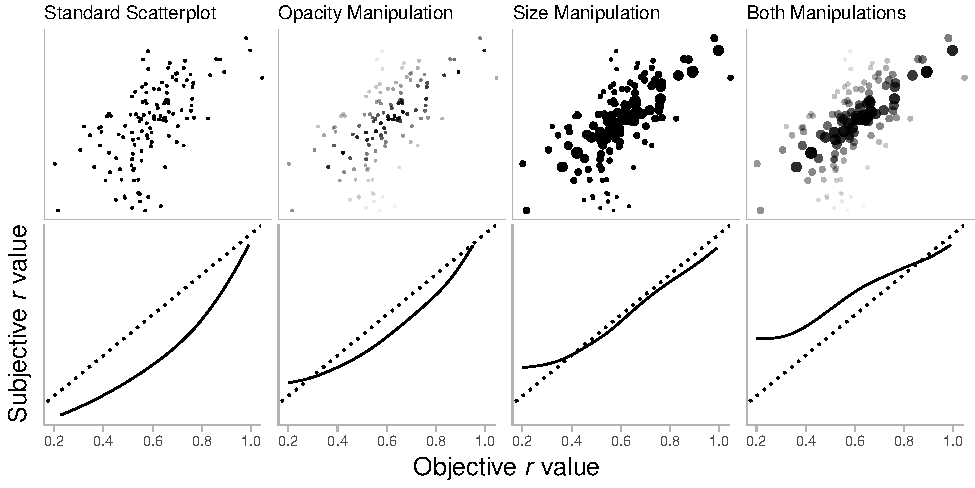
\includegraphics[width=1\textwidth,height=\textheight]{beliefs_alternative_scatterplots_files/figure-pdf/fig-previous-manipulations-1.pdf}

}

\caption{\label{fig-previous-manipulations}Top row: Examples of
scatterplot manipulations from previous work using an \textit{r} value
of 0.6. Bottom row: the corresponding correlation estimation behaviour
across values of \textit{r} between 0.2 and 0.99. The dashed diagonal
line represents perfectly accurate estimation, while the solid line is
what is observed when participants are asked to estimate correlation.}

\end{figure*}%

\subsection{Perception \& Cognition in Data
Visualization}\label{sec-perception-cognition}

Interacting with data visualization is a complex process involving
bottom-up and top-down mechanisms
\citep{shah_2011, franconeri_2021, xiong_2022}. Previous work
investigating alternative scatterplot designs has predominantly focused
on perceptual factors and mechanisms; here we introduce the potential
for top-down effects to bias participants. Recent work has established
that scatterplots are able to induce different levels of belief change
in viewers \citep{karduni_2020, markant_2023}; this may depend on
factors such as prior belief strength, attitudes, and the presence or
absence of uncertainty visualizations. Accordingly, our pre-study is
essential for isolating our variable of interest, the alternative
scatterplot design. Data visualization does not take place without
context, and so the investigation of top-down effects is critical for
providing designers with the tools to design visualizations that work as
intended in the field. We therefore present a two-experiment study
investigating the propensity for recently established scatterplot
visualization techniques to bias participants' beliefs about the levels
of relatedness between variables.

\section{General Methods}\label{sec-general-methods}

In this section, we discuss our general research methods, including our
implementations of open research practices and our approach to and
justification for crowdsourcing.

\subsection{Open Research}\label{sec-open-research}

Both our pre- and main studies were conducted according to the
principles of open and reproducible research \citep{ayris_2018}. We
pre-registered hypotheses and analysis plans with the Open Science
Framework (OSF) for the pre-study\footnote{https://osf.io/xuf4d} and the
main experiment\footnote{https://osf.io/anmez}. All data and analysis
code are included in a GitHub repository\footnote{https://github.com/gjpstrain/beliefs\_alternative\_scatterplots}.
This repository contains instructions for building a Docker container
\citep{merkel_2014} that reproduces the computational environment in
which the paper was written. This allows for full replication of
stimuli, figures, analyses, and the paper itself. Ethical approval was
granted by the University of Manchester's Computer Science departmental
ethics panel (Ref: 2024-19426-33788).

\subsection{Crowdsourcing}\label{sec-crowdsourcing}

While much prior work into correlation perception in scatterplots has
taken place in person, there is precedent for work that explores
cognition and perception to take place online using crowdsourced
participants \citep{xiong_2022}. Crowdsourcing affords us recruitment of
samples from across our lay population of interest, and it is
considerably quicker and less expensive than in-person testing. Previous
work has reported issues of data quality and skewed demographics
\citep{chmielewski_2020, charalambides_2021, peer_2021}, so we follow
published guidelines \citep{peer_2021} to give us the best chance of
collecting high-quality data. We use the Prolific platform
\citep{prolific} with strict pre-screening criteria; participants were
required to have completed at least 100 studies using Prolific and were
required to have a Prolific score of 100, representing a 99\% approval
rate.

\section{Pre-Study: Investigating Beliefs About Relatedness
Statements}\label{sec-pre-study}

The goal of the present study is to investigate to what extent a novel
scatterplot design can alter participants' beliefs about correlations.
Due to our targeting of lay populations, and the authors' prior
experience with lay participants failing to understand the term
``correlation'' (although not the concept), we elected to operationalize
correlation for our participants as ``strength of relatedness''. There
is evidence that belief change can be affected by prior beliefs and
attitudes \citep{xiong_2022, markant_2023}, and that emotion, including
the content of a visualization \citep{phelps_2006, harrison_2013} and
the emotional state of a participant \citep{thoresen_2016} can have
perceptual and cognitive effects on participants. We were unable to find
resources for correlative statements that included ratings for belief
strength and emotional valence, so elected to create our own. To control
for these factors as much as possible in the main experiment, we ran our
pre-study with the intent of finding a correlative statement that was
matched on emotional valence and level of belief strength. Instead of
creating these statements ourselves, we chose to streamline the process
by using the ChatGPT4 Large Language Model \citep{chat_gpt}. We used the
following prompt:

\begin{quotation}
    ``Generate 100 statements that describe the correlation between two variables, such as:
     "X is associated with a higher level of Y" or
     "As X increases, Y increases".
    Try to match all the statements on emotionality.''
    
\end{quotation}

The full list of these statements can be found in the supplemental
materials. Two authors rated each statement on emotional valence and
belief about strength of relatedness using Likert scales from 1 to 7.
Both statement emotional valence and strength of relatedness were
anchored at points 1 and 7: \emph{Very Negative} and \emph{Very
Positive} for the former, and \emph{Not Related At All} and
\emph{Strongly Related} for the latter. All other points were
unlabelled. We calculated a quadratic weighted Cohen's Kappa between the
two raters using the \textbf{irr} package (version 0.84.1 \citep{irr})
to penalize larger magnitude disagreements more harshly. We found
agreement above chance for both emotional valence (\(\kappa\) = 0.49,
\emph{p} \textless{} .001) and strength of relatedness (\(\kappa\) =
0.51, \emph{p} \textless{} .001), indicating moderate levels of
agreement in both cases \citep{cohen_1968, fleiss_1969}. Following this,
we selected strongly and weakly correlated statements with the highest
level of absolute agreement, resulting in 14 strongly correlated
statements and 11 weakly correlated statements that can be seen in the
supplemental materials. We then tested these 25 statements with a
representative UK sample to ascertain consensus on both statement
emotionality and strength of relatedness. Doing so allows us to minimize
the impact of these factors when we analyse the effects of alternative
scatterplot design on the propensity for belief change in our main
experiment. We hypothesized that:

\begin{itemize}
\tightlist
\item
  H1: there will be a significant difference in the average ratings of
  emotional valence between statements.\footnote{The pre-registration
    for this hypothesis refers to ``emotionality''. In response to
    reviewer comments, we have clarified that we tested emotional
    valence, and have therefore used this wording here.}
\item
  H2: there will be a significant difference in the average ratings of
  strength of relatedness between statements.
\end{itemize}

\subsection{Method}\label{sec-method-pre}

\subsubsection{Participants}\label{sec-participants-pre}

100 participants were recruited using the Prolific platform
\citep{prolific}. English fluency and UK residency were required for
participation, as our main experiment relied on familiarity with data
visualizations from a popular British news source. In addition to 25
experimental items, we included six attention check items that
instructed participants to ignore the scatterplot and provide specific
answers. No participants failed more than 2 out of 6 attention check
items, and therefore data from all 100 were included in the full
analysis (52 male and 48 female). Participants' mean age was 41.1
(\emph{SD} = 12.3). The average time taken to complete the survey was
7.6 minutes (\emph{SD} = 2.9 minutes).

\subsubsection{Design}\label{sec-design-pre}

Each participant saw all survey items (see supplemental material), along
with the six attention check items, in a fully randomized order. All
experimental code, materials, and instructions are hosted on
GitLab\footnote{https://gitlab.pavlovia.org/Strain/beliefs\_scatterplots\_pretest}.

\subsubsection{Procedure}\label{sec-procedure-pre}

The experiment was built using Psychopy \citep{pierce_2019} and hosted
on Pavlovia.org. Participants were permitted to complete the experiment
using a phone, tablet, desktop, or laptop computer. Participants were
first shown the participant information sheet and were asked to provide
consent through key presses in response to consent statements. They were
asked to provide their age in a free text box, followed by their gender
identity. Participants were told that they would be asked to read
statements about the relatedness between a pair of variables, after
which they would have to answer some questions. To familiarize
themselves with the sliders, they were asked to complete a practice
round in response to the statement: ``As participation in online
experiments increases, society becomes happier.'' Following each
statement, a pair of Likert scales were presented labelled ``Statement
Emotionality'' and ``Strength of Relatedness''; these scales were
identical to those used by the researchers in
Section~\ref{sec-pre-study}.

\subsection{Results}\label{sec-results-pre}

All analyses were conducted using R (version 4.4.0)` \citep{rcore}). We
use the \textbf{irr} package to calculate Fleiss' Kappa to measure
interrater agreement on statement emotional valence and strength of
relatedness for the 25 experimental items. This analysis revealed that
participants agreed above chance on statement emotional valence
(\(\kappa\) = 0.07, \emph{p} \textless{} .001) and strength of
relatedness (\(\kappa\) = 0.06, \emph{p} \textless{} .001).

\subsection{Selecting Statements for the Main
Experiment}\label{sec-selecting-statements}

To control for the potential effects of statement emotionality in the
main experiment, we first select statements that represent neutral
emotional valence. Statements with average emotionality ratings between
3 and 5 are statements 2, 10, 22, 16, and 23, which can be seen in
Table~\ref{tbl-candidate-statements}. To ascertain which statements
represent the greatest consensus, we add standard deviations in ratings
for statement emotional valence and strength of relatedness. Due to
concerns about experimental power, and in line with evidence that
propensity for belief change is highest when prior beliefs are not
strongly held \citep{xiong_2022, markant_2023}, we elected at this point
to test only the statement corresponding to weak beliefs about the
strength of relatedness between the variables in question. We therefore
test statement number 22, ``Higher consumption of spicy foods is
associated with a lower risk of certain types of cancer'', however we
modify the wording so that the variables (food consumption and cancer
risk) are positively correlated, as while the manipulations we use in
the alternative scatterplot condition can affect estimates of
correlation in positively correlated scatterplots, no work regarding the
effects of these manipulations in negatively correlated scatterplots has
been completed.

\begin{table}

\caption{\label{tbl-candidate-statements}Statements with neutral average
emotional valence ratings.}

\centering{

\centering
\resizebox{\ifdim\width>\linewidth\linewidth\else\width\fi}{!}{
\begin{tabular}[t]{r>{\raggedright\arraybackslash}p{7.5cm}}
\toprule
Item & Statement\\
\midrule
2 & As caffeine consumption increases, so does the average heart rate.\\
10 & Higher sugar consumption is associated with an increased risk of dental cavities.\\
16 & As the amount of sleep decreases, the risk of obesity increases.\\
22 & Higher consumption of spicy foods is associated with a lower risk of certain types of cancer.\\
23 & Greater adherence to a Mediterranean diet is linked to a lower risk of neurodegenerative diseases.\\
\bottomrule
\end{tabular}}

}

\end{table}%

\subsection{Discussion}\label{sec-discussion-pre}

Fleiss' Kappa values for interrater agreement on both statement
emotional valence and strength of correlation scales are low (\(\kappa\)
= 0.07 and \(\kappa\) = 0.06 respectively), however do exceed that which
would be expected by chance. In light of this we do not make decisions
regarding which statement to use based on the values of Fleiss' Kappa
observed, but rather on the standard deviations of ratings across all
raters. We also test statement emotionality and strength of correlation
with participants in the main study and include these ratings as part of
our analyses.

\section{Main Study: Potential for Belief Change Using Alternative
Scatterplots}\label{sec-main-study}

We test the statement that exhibited the lowest average level of belief
about strength of relatedness and the 2\textsuperscript{nd} highest
level of consensus. Modified for directionality, this statement is
therefore: ``Higher consumption of plain (non-spicy) foods is associated
with a higher risk of certain types of cancer.'' To give ourselves the
best chance of detecting an effect of viewing alternative scatterplots,
we elected to design our scatterplots based on a popular British news
source and to falsely credit the data as being provided by the British
National Health Service (NHS). Participants were informed that said news
source had requested that their identity be obscured. They were
debriefed that this was not the case, and that the data were fictional,
following completion of the experiment. Based on previous evidence that
beliefs can change after viewing data visualizations
\citep{karduni_2020, markant_2023}, and that scatterplots employing the
point size and opacity manipulations detailed in
Section~\ref{sec-scatterplots} are able to affect perceptual estimates,
we make the following hypotheses:

\subsection{Hypotheses}\label{hypotheses}

\begin{itemize}
\tightlist
\item
  H1: there will be a significant difference between ratings of strength
  of relatedness made before and after participants viewed scatterplots
  in either the standard or alternative conditions.
\item
  H2: this difference will be greatest when participants are exposed to
  scatterplots in the alternative scatterplot condition.
\end{itemize}

We also undertake exploratory investigations taking into account
participants' scores on a defensive confidence test, their scores on a
graph literacy test, and each participant's rating of the emotional
valence of the correlative statement used. Analysis including each of
these factors can be found in Section~\ref{sec-add-analyses}, and we
justify their inclusion below.

\subsubsection{Defensive Confidence}\label{sec-def-con}

In line with evidence that those who are more confident in their ability
to defend their own positions are more susceptible to having those
positions changed \citep{albarracin_2004}, we measured participants'
defensive confidence using Albarracín and Mitchell's
\citep{albarracin_2004} 12-item scale. This scale is replicated from
previous work in the supplemental material, and has been utilized more
recently \citep{markant_2023} to explore the potential for attitude
change specifically with regard to correlations in scatterplots.
Participants provide answers to the 12 scale items using a 5-point
Likert scale anchored at points 1 (\emph{not at all characteristic of
me}) and 5 (\emph{extremely characteristic of me}), with all other
points being unlabelled. Analysis including participants' defensive
confidence scores is included in
Section~\ref{sec-add-analyses-discussion}.

\subsubsection{Graph Literacy}\label{sec-graph-lit}

Previous work testing the systematic adjustment of point opacity and
size in scatterplots has found no effect of graph literacy on
participants' estimates of positive correlation
\citep{strain_2023, strain_2023b, strain_2024}. Despite this, we elect
to include the test here due to the higher cognitive load of the current
task, along with evidence that graph literacy may affect performance on
more cognitively demanding visualization tasks
\citep{canham_2010, okan_2012}. Additionally, the graph literacy test we
use \citep{garcia_2016} is extremely short; in the present study, this
took participants an average of 27 seconds (\emph{SD} = 16 seconds).

\subsubsection{Emotionality}\label{sec-emotionality}

As discussed in Section~\ref{sec-pre-study}, the emotional content of a
visualization and the emotional state of participants may have cognitive
and perceptual effects on performance in visualization tasks
\citep{phelps_2006, harrison_2013, thoresen_2016}; this was the primary
intention behind performing the pre-study. Nonetheless, we cannot be
certain that each participant considers the emotional content of our
chosen correlative statement to be the same. To account for these
potential individual differences, we also collect participants' ratings
of emotional valence during the main study.

\subsection{Stimuli}\label{sec-stimuli-main}

Having selected a correlative statement describing a weak relationship
and with a high level of consensus between participants in the
pre-study, we used \textbf{ggplot2} (version 3.5.1 \citep{ggplot}) in R
to create our stimuli; scripts for the creation of stimuli can be found
in the repository associated with this project. As our statement was
rated as describing a low level of relatedness, we utilize scatterplots
that describe a strong relationship (0.6 \textless{} \emph{r}
\textless{} 0.99) to induce belief change. Our plots were created in
line with guidance provided by previous research; plots in the
alternative scatterplot condition feature points that decrease in size
and opacity as a function of residual distance, as this has been shown
to increase estimates of correlation in positively correlated
scatterplots \citep{strain_2023, strain_2023b, strain_2024}. We used 45
values of \emph{r} uniformly distributed between 0.6 and 0.99 to create
45 scatterplots for each condition. Examples of stimuli using an
\emph{r} value of 0.6 for both the standard and alternative scatterplot
conditions can be seen in Figure~\ref{fig-main-examples}.

\begin{figure*}

\centering{

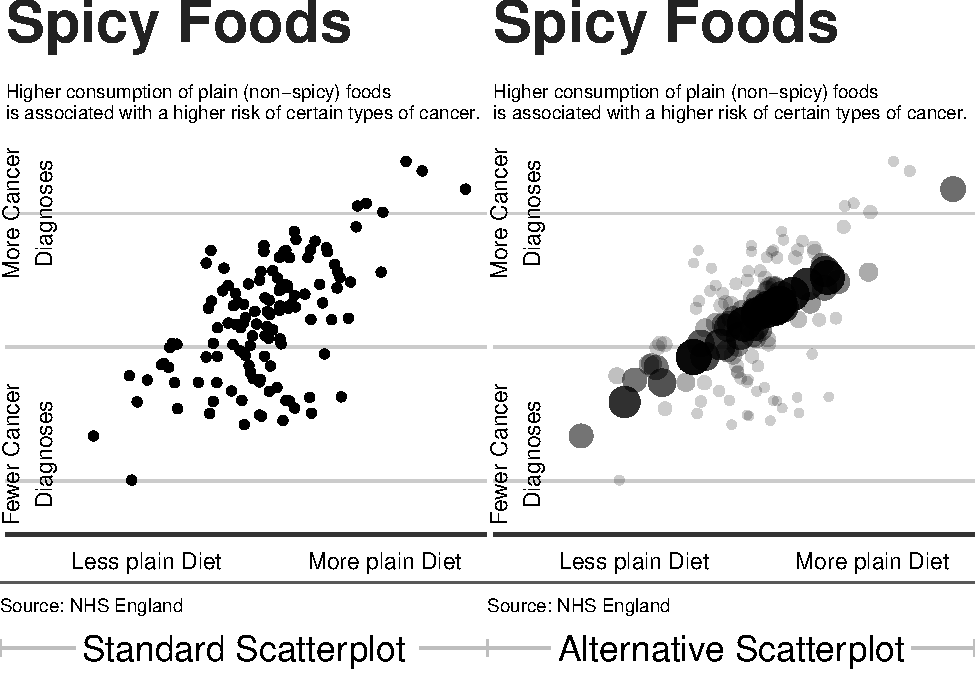
\includegraphics[width=1\textwidth,height=\textheight]{beliefs_alternative_scatterplots_files/figure-pdf/fig-main-examples-1.pdf}

}

\caption{\label{fig-main-examples}Examples of the experimental stimuli
used with an \textit{r} value of 0.6.}

\end{figure*}%

\subsection{Method}\label{sec-method-main}

\subsubsection{Participants}\label{sec-participants-main}

Participants were recruited using Prolific \citep{prolific}. English
fluency and UK residency were required for participation, as well as
normal or corrected-to-normal vision, and having not participated in any
of our previous studies regarding correlation perception in scatterplots
\citep{strain_2023, strain_2023b, strain_2024}. Data were collected from
77 participants for each condition. 2 participants failed more than 2
out of 4 attention check questions for each condition, meaning their
data were excluded per pre-registration stipulations. Data from the
remaining 150 participants were included in the full analysis (73 male,
73 female, and 4 non-binary). Participants' mean age was 39.3 (\emph{SD}
= 11.5). Participants' mean graph literacy score was 21.3 (\emph{SD} =
4.3) out of 30, their mean defensive confidence score was 43 (\emph{SD}
= 6.8) out of 60, and their mean rating of statement emotional valence
was 2.9 (\emph{SD} = 1.3) on a 7-point Likert scale. On average,
participants took 14.2 minutes to complete the experiment (\emph{SD} =
6.41).

\subsubsection{Design}\label{sec-design-main}

We employed a between-participants design. Each participant was randomly
assigned to either group A, in which case they viewed standard
scatterplots, or group B, in which they viewed alternative scatterplots
designed deliberately to elicit higher levels of belief change.
Participants saw all 45 experimental items for their group, along with 4
attention check items, in a fully randomized order. Our dependent
variable was the level of belief change induced by viewing the
scatterplot visualizations, so participants were tested on how strongly
related they believed the variables described by the correlative
statement were both \textbf{before} and \textbf{after} viewing the
experimental items. All experimental code, materials, and instructions
are hosted on GitLab as two separate experiments \footnote{https://gitlab.pavlovia.org/Strain/atypical\_scatterplots\_main\_t}
\footnote{https://gitlab.pavlovia.org/Strain/atypical\_scatterplots\_main\_a}.

\subsubsection{Procedure}\label{sec-procedure-main}

We used PsychoPy \citep{pierce_2019} to build our experiment and
Pavlovia.org to host it. Participants were permitted to complete the
experiment on a desktop or laptop computer. We elected to prevent
participants from using a phone or tablet to complete the experiment as
there is evidence that differences in the on-screen sizes of data
visualizations can alter perceptions \citep{cleveland_1982}.
Participants were first shown the participant information sheet and
asked to provide consent through key presses in response to consent
statements, after which they were asked to provide their age and gender
identity. Participants then completed the 12-item Defensive Confidence
scale described by Albarracín and Mitchell \citep{albarracin_2004} and
the 5-item Subjective Graph Literacy scale \citep{garcia_2016}
\footnote{The inclusion of this scale was not specified in the
  pre-registration.}. To give legitimacy to our data visualizations with
the hope of maximizing any potential belief change, participants were
told that the graphs were taken from a well-known British news source,
but that the identity of this source had been obscured. To promote
engagement with the visualizations, participants were instructed to use
a slider to estimate the correlation displayed in each scatterplot; no
hypotheses were made based on these data and therefore we do not analyse
them further. Following instructions, which included descriptions of
scatterplots and Pearson's \emph{r}, participants had a chance to
practice using the slider, before being asked to indicate their beliefs
about emotional valence and the strength of relatedness between the
variables described in our chosen statement. We captured these data
using Likert scales identical to those described in
Section~\ref{sec-pre-study}. After completing the experimental trials,
participants were tested again on their beliefs about strength of
relatedness and then debriefed that the data they were shown were
fictional. Interspersed among the experimental items were 4 attention
check trials which explicitly asked participants to set the slider to 0
or 1.

\subsection{Results}\label{sec-results-main}

All analyses were conducted using R (version 4.4.2 \citep{rcore}).
Likert scales capture whether one rating is higher or lower than
another, however they do not quantify the difference between levels of
rating. Metric modelling assuming equal levels of difference between
ratings, such as linear regression, is therefore inappropriate
\citep{liddell_2018}. In light of this, we use the \textbf{ordinal}
package (version 2023.12-4.1 \citep{ordinal}) to build cumulative link
mixed effects models to analyse Likert scale data \footnote{Our
  pre-registration specified linear mixed effects models (metric).
  Conclusions are identical when using said models, and code for this
  analysis is included in the repository associated with this paper.}.
We use the \textbf{buildmer} (version 2.11 \citep{buildmer}) package to
automate selection of the random effects structure; we provide a maximal
model, which includes random intercepts for participants, and
\textbf{buildmer} identifies the most complex model that successfully
converges. We present odds ratios and equivalent Cohen's \emph{d} effect
sizes that were calculated using the \textbf{effectsize} package
(version 0.8.9 \citep{effectsize}).

To test the first hypothesis, that ratings of strength of relatedness
would be different before and after participants viewed experimental
items, we build a model whereby the rating of strength of relatedness
the participant made is predicted by whether it was made \textbf{before}
or \textbf{after} viewing the experimental items. Our first hypothesis
was supported; there was a significant difference in ratings of strength
of relatedness made before and after participants viewed the
experimental plots. A likelihood ratio test revealed that the model
including time of rating as a predictor explained significantly more
variance than the null (\(\chi^2\)(1) = 8,046.95, \emph{p} \textless{}
.001). This model has random intercepts for participants. Statistical
testing providing support for this hypothesis is shown in
Table~\ref{tbl-rating-time}. Figure~\ref{fig-descriptives} shows means
and dot plots for ratings of strength of relatedness made before and
after viewing scatterplots in either the standard or alternative
condition.

\begin{table}

\caption{\label{tbl-rating-time}Statistics for the significant main
effect of rating time. Odds ratio and the equivalent Cohen's \textit{d}
value is also supplied.}

\centering{

\begin{tabular}[t]{lrrrlrr}
\toprule
  & Estimate & Standard Error & Z-value & \textit{p} & Odds Ratio & Cohen's \textit{d}\\
\midrule
Rating Time & 3.77 & 0.049 & 76.63 & <0.001 & 43.2 & 2.08\\
\bottomrule
\end{tabular}

}

\end{table}%

\begin{figure*}

\centering{

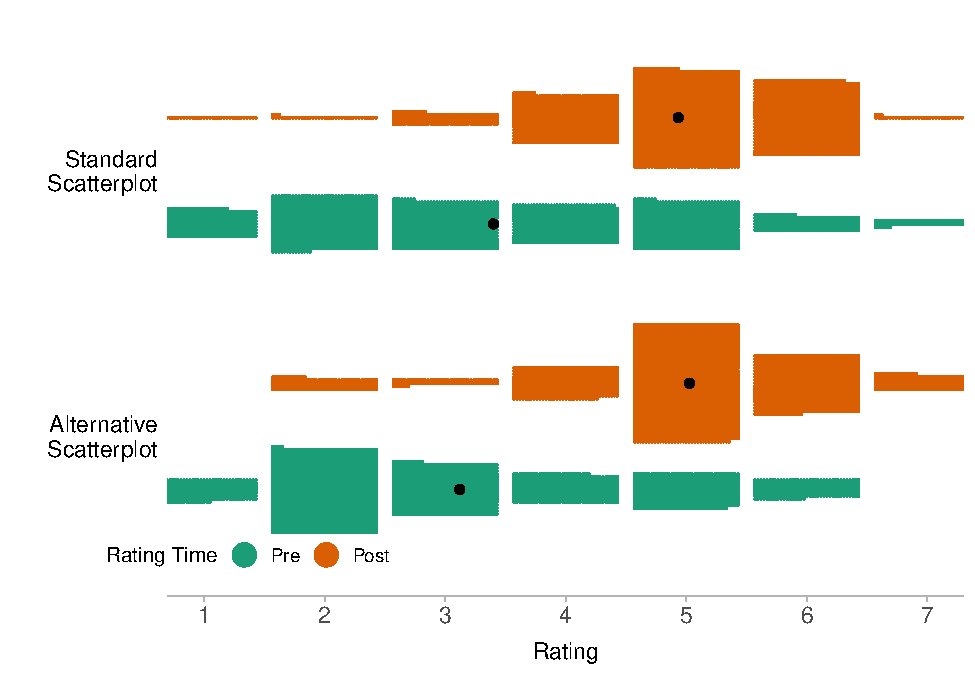
\includegraphics[width=1\textwidth,height=\textheight]{beliefs_alternative_scatterplots_files/figure-pdf/fig-descriptives-1.pdf}

}

\caption{\label{fig-descriptives}Dot plots for pre- and post-plot
viewing ratings of strength of relatedness for standard and alternative
scatterplot conditions. Mean ratings are also shown as points.}

\end{figure*}%

Our second hypothesis, that the difference between ratings of strength
of relatedness before and after viewing experimental plots would be
greater when participants were assigned to the alternative scatterplot
condition, also received support. Treatment coding was used for each of
the experimental factors of rating time (pre- or post-) and condition,
which allows us to compare means of ratings made after viewing the
experimental items directly to those made before viewing. We built a
cumulative link mixed effects model whereby the rating of strength of
relatedness the participant made was predicted by the condition the
participant was assigned to and the time they made the rating. A
likelihood ratio test revealed that the model including condition and
rating time as predictors explained significantly more variance than the
null (\(F\)(3) = 8,151.94, \emph{p} \textless{} .001). This model had
random intercepts for participants. We again found a main effect of
rating time, found no main effect of condition, and found an interaction
between rating time and condition. Test statistics, along with odds
ratios and equivalent Cohen's \emph{d} effect sizes can be seen in
Table~\ref{tbl-condition-interact}. The estimate for the interaction
corresponds to the difference-in-difference between ratings made pre-
and post-viewing for standard and alternative scatterplots. This
difference-in-difference is visualized in
Figure~\ref{fig-difference-descriptive}; the difference in ratings
between pre- and post-plot viewing times is greater for the participants
who were exposed to the alternative scatterplot condition.

\begin{figure*}

\centering{

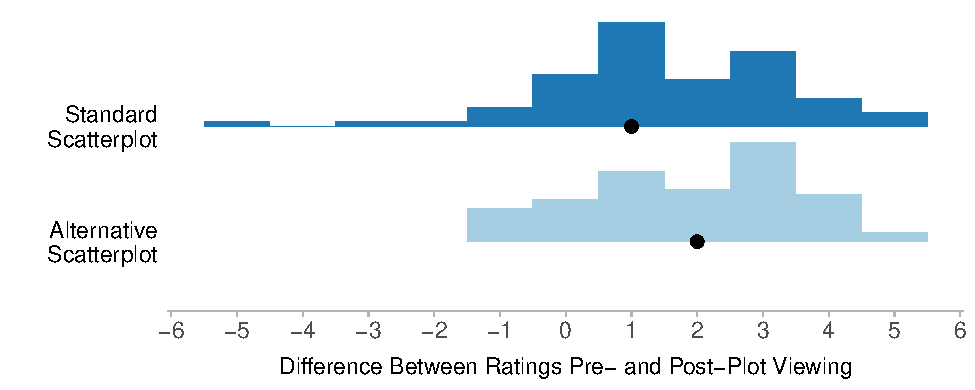
\includegraphics{beliefs_alternative_scatterplots_files/figure-pdf/fig-difference-descriptive-1.pdf}

}

\caption{\label{fig-difference-descriptive}Histograms illustrating the
magnitudes of the difference between pre- and post-plot viewing ratings
of strength of relatedness. Median values are plotted as points.}

\end{figure*}%

\begin{table}

\caption{\label{tbl-condition-interact}Statistics for the significant
main effect of rating time and the significant interaction between
rating time and condition on the difference between pre- and
post-scatterplot viewing ratings for standard and alternative plots.
Odds ratios and equivalent Cohen's \emph{d} effect sizes are also
shown.}

\centering{

\begin{tabular}[t]{lrrrlrr}
\toprule
  & Estimate & Standard Error & Z-value & \textit{p} & Odds Ratio & Cohen's \textit{d}\\
\midrule
Rating Time & 4.15 & 0.063 & 66.34 & <0.001 & 63.33 & 2.29\\
Condition & 0.49 & 0.390 & 1.25 & 0.211 & 1.63 & 0.27\\
Rating Time x Condition & -0.72 & 0.071 & -10.22 & <0.001 & 2.06 & 0.40\\
\bottomrule
\end{tabular}

}

\end{table}%

\subsubsection{Additional Analyses}\label{sec-add-analyses}

We also found effects of participants' scores on the defensive
confidence test (\(F\)(4) = 69.73, \emph{p} \textless{} .001),
participants' scores on the graph literacy test (\(F\)(4) = 42.66,
\emph{p} \textless{} .001), and of how emotionally valent participants
rated the chosen correlative statement before beginning the block of
trials (\(F\)(4) = 43.51, \emph{p} \textless{} .001). We discuss the
interactions between the main effect and graph literacy, defensive
confidence, and statement emotional valence in
Section~\ref{sec-add-analyses-discussion}.

\subsection{Discussion}\label{sec-main-discussion}

Both of our hypotheses were supported in this experiment. Participants
reliably updated their beliefs after viewing scatterplots, and the
difference between pre- and post-viewing beliefs was greatest for the
participants who viewed scatterplots in the alternative condition. These
results suggest that the effects described in previous work can go
beyond perception and have impacts on higher-level cognitions,
specifically, participants' beliefs about strength of relatedness. These
findings are encouraging for data visualization designers who wish to
design scatterplots such that correlation perception more closely
matches the underlying statistics, however further work is required
before developing guidelines for the use of alternative scatterplot
designs with regards to producing more persuasive visualizations.

\subsubsection{Graph Literacy, Defensive Confidence, and Statement
Emotionality}\label{sec-add-analyses-discussion}

\begin{figure*}

\centering{

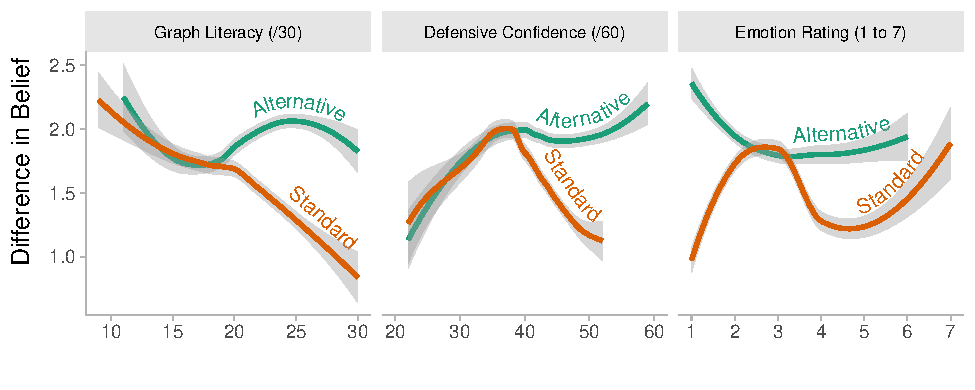
\includegraphics{beliefs_alternative_scatterplots_files/figure-pdf/fig-add-analyses-plots-1.pdf}

}

\caption{\label{fig-add-analyses-plots}Illustrating how differences in
beliefs about strength of relatedness change as a function of
participants' scores on the graph literacy test (left), their scores on
the defensive confidence test (center), and their ratings of statement
emotionality (right). Localled smoothed curves with 95\% CI ribbons are
shown separately for standard and alternative scatterplot viewing
conditions. Lower ratings of Difference in Beliefs (\(y\) axis)
corresponds to lower levels of belief change between pre- and
post-scatterplot viewing times.}

\end{figure*}%

Mean differences in pre- and post-plot viewing ratings of strength of
relatedness by Subjective Graph Literacy score can be seen in
Figure~\ref{fig-add-analyses-plots}. Generally, participants with higher
scores on a graph literacy test experienced smaller changes in their
ratings of strength of relatedness. This is in line with previous work
suggesting that those with higher levels of graph or visualization
literacy show better performance in inference tasks related to
visualizations \citep{canham_2010}, are more capable of describing
effects that visualizations aim to communicate \citep{shah_2011}, and
can preferentially attend to relevant features of visualizations to a
greater degree \citep{okan_2016}, than those with lower levels of graph
literacy. In the present study, we provide evidence that those with
greater levels of graph literacy are \emph{less susceptible} to having
their beliefs changed by visualizations. The use of the alternative plot
manipulation largely removes this effect, suggesting that there is less
systematic reliance on graph literacy when participants are faced with
an unfamiliar data visualization.

We observe an opposing pattern of results when examining the effects of
defensive confidence on participants' propensity for belief change.
Generally, participants with higher scores on the defensive confidence
test experienced greater levels of belief change. This is in line with
evidence that those who are more confident in their ability to defend
their own beliefs are more liable to having those beliefs changed in
light of evidence \citep{albarracin_2004}. This effect has previously
been explained as being due to those with a greater degree of confidence
in their own ability to defend their ideas engaging with information
with lower levels of attention to the fact it opposes their beliefs. The
present study provides additional evidence in favour of this phenomenon.
While the general pattern of results is expected based on previous work,
the interaction present between defensive confidence and scatterplot
condition is novel. It would appear that despite following the normal
pattern of results for low to moderate levels of defensive confidence,
those participants who viewed the standard scatterplots experienced a
drop in belief change as defensive confidence increased past
\textasciitilde{} 36/60. We suggest that the unfamiliar nature of the
alternative scatterplots was protective against an unexpected behaviour
whereby very high levels of defensive confidence decrease susceptibility
to belief change.

The effect of statement emotional valence on belief change is also
illustrated in Figure~\ref{fig-add-analyses-plots}. There is a broad
research space regarding emotionality and data visualization
\citep{lan_2023}, and it is clear from previous work that emotion
affects perception, cognition, and behavior
\citep{phelps_2006, harrison_2013, thoresen_2016} regarding to data
visualization. Harrison et al. \citep{harrison_2013} found that
participants who were positively primed performed better on a low-level
visual judgement task compared to negative primes. Comparison of this
work to the current is difficult, as \emph{success} on our task is hard
to define.

Further experimental work is required to provide more comprehensive
explanations for the interactive effects of graph literacy, defensive
confidence, and statement emotionality in the current experimental
paradigm.

\section{General Discussion}\label{sec-general-discussion}

The most parsimonious explanation for the results we observe in the
present study is as follows; things that \emph{look} more related will
be \emph{judged} as being more related, and are therefore \emph{more}
able to change beliefs about the levels of relatedness between
variables. Given the frequent real-world usage of scatterplots, and the
role of data visualizations in decision-making, it is particularly
important to empirically test whether perceptual effects may be extended
into a cognitive space to influence beliefs. Doing so is a necessary
step in broadening the data visualization design space and bringing
novel designs closer towards use cases with the potential for real-world
consequences while maintaining a strong foundation of experimental
evidence. Having controlled as far as possible for factors such as
emotional content, the consensus on how related the variables in
question were, and the general design (bar the points themselves) of the
scatterplot, we can conclude with strong evidence that alternative
scatterplot design was responsible for increasing the level of belief
change amongst participants.

An alternative (although not competing) explanation for the results we
have seen here comes from recent work on the incorporation of
uncertainty visualizations in scatterplots. Karduni et al.
\citep{karduni_2020} found in 2020 that visualizations that encode
uncertainty produce lower levels of belief change compared to those that
do not. The alternative scatterplot design we employed can be thought of
as masking some of the uncertainty inherent in a scatterplot point cloud
by reducing the salience of the most exterior points.

Previous work has provided support for the idea that it is the shape of
the point cloud, more specifically, the width of the probability
distribution it represents, that drives correlation perception in
scatterplots. If this mechanism were valid, our results would be
expected. These results are broadly consequential. For data
visualization designers, they provide strong evidence that utilizing the
alternative scatterplot designs described here and in previous work can
affect beliefs about levels of relatedness without requiring the removal
of data. For researchers, these results pave the way for work in a
number of directions, which we discuss in Section~\ref{sec-future-work}.

\section{Future Work}\label{sec-future-work}

Because alternative scatterplot designs have not been tested before with
regard to belief change, we elected to design our study with the
intention of capturing effects, should they exist. This meant that our
design was simple; we did not investigate multiple correlative
statements, the propensity for strongly held beliefs to be changed, nor
the effect of topics with strong or polarized emotional components. We
chose to use a simple, blunt measure of belief about relatedness, and
did not investigate variations within the alternative scatterplot design
space, such as using different values of equation 1, or using opacity or
size manipulations in isolation. Each of these components deserves
study, and each is ripe for future work to investigate the contributions
of each factor to the effects we have seen here.

In Section~\ref{sec-add-analyses-discussion}, we describe the effects
that graph literacy, defensive confidence, and participants' ratings of
the emotionality of the correlative statement have on the propensity for
belief change. Future work may wish to investigate these factors, along
with others that affect perceptions of correlation, such as educational
background or spatial abilities \citep{tandon_2024}. Xiong et al.
\citep{xiong_2022} describe how correlation estimation may differ
according to the context the data are presented in; this could be
extended to instead investigate statements with differing emotional
contents and how alternative scatterplot designs might interact with
emotional valence. Similarly, selecting matched participant groups with
low or high graph literacy or defensive confidence would facilitate
understanding of how we might use alternative designs to cater for
people with different levels of experience, or who differ in terms of
their faith in their own ideas and abilities.

Previous works investigating beliefs with regard to correlation
estimation have made distinctions between beliefs and attitudes
\citep{xiong_2022, markant_2023}. We elected not to do so due to our
utilization of alternative designs. Markant et al. \citep{markant_2023}
found that while beliefs about correlations changed in participants as a
result of interaction with scatterplots, attitudes did not. Future work
may wish to investigate whether this finding would persist with
scatterplots utilizing the alternative designs described here. Finally,
while changing perceptions, beliefs, and attitudes are promising early
steps, changing people's behaviours would be the real test of the power
of alternative visualization techniques; while this may be difficult to
study, future work should investigate whether what we have found here
may be used to induce behaviour change.

\section{Limitations}\label{sec-limitations}

Our commitment to finding an effect, should one exist, is also our
biggest limitation. The exploratory nature of the work results in us
being unable to comment specifically on how different forms of size and
opacity manipulation in scatterplots may change beliefs in different
ways, although addressing this using the framework we present here would
be simple to accomplish. To date, there has been no qualitative work
performed on alternative scatterplot designs such as those we utilize
here; it may be that any perceptual or cognitive benefits are outweighed
by distrust or unfamiliarity with novel designs. We chose to use a
simple, blunt, 7-point Likert scale. While we argue that this is not
particularly problematic given that we intended only to find an effect
(and succeeded in that), future work may wish to use techniques that
provide further scope for analysis, such as the graphical elicitation
method developed by Karduni et al. \citep{karduni_2020, karduni_2023}.

\section{Conclusion}\label{sec-conclusion}

We investigated the effects of alternative scatterplot designs that vary
the opacities and sizes of points as a function of their distance from
the regression line on the propensity for belief change following
scatterplot visualization viewing. We presented these designs, and
corresponding standard scatterplots, as if they were part of news items,
and used a real-world variable pair that had been selected by our
population of interest as being representative of a weakly-held,
emotionally neutral correlation. We found that participants who viewed
scatterplots employing alternative designs experienced greater levels of
belief change compared to those who viewed standard plots. In addition,
we found small interactive effects of a number of participant
characteristics. Our results suggest that visualization techniques that
have previously been employed to improve perception amongst participants
are deserving of study with regards to their potential to change
beliefs.

\bibliographystyle{ACM-Reference-Format}
\bibliography{alternative-scatterplots.bib}

%% begin pandoc before-bib
%% end pandoc before-bib
%% begin pandoc biblio
%% end pandoc biblio
%% begin pandoc include-after
%% end pandoc include-after
%% begin pandoc after-body
%% end pandoc after-body

\end{document}
\endinput
%%
%% End of file `sample-manuscript.tex'.
